\documentclass[lettersize,journal]{IEEEtran}
\usepackage{tikz}
\usetikzlibrary{shapes,arrows,positioning}

\begin{document}

% Upper Half (Encoder)
\begin{figure*}[t]
\centering
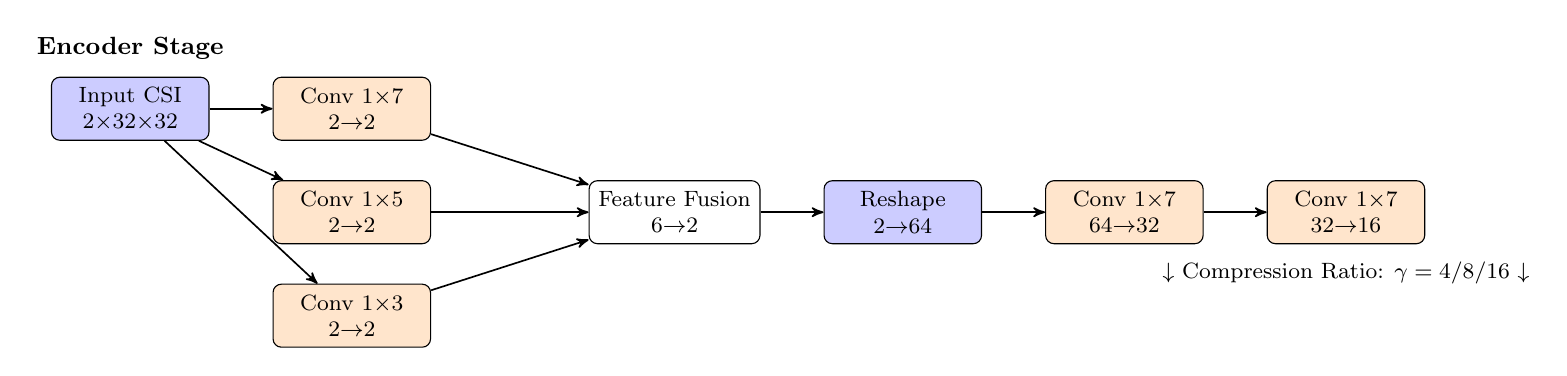
\begin{tikzpicture}[
    node distance=0.5cm and 0.8cm,
    block/.style={draw, fill=white, rectangle, minimum width=2cm, minimum height=0.8cm, font=\footnotesize, align=center, rounded corners=3pt},
    conv/.style={block, fill=orange!20},
    compress/.style={block, fill=blue!20},
    arrow/.style={->, >=stealth', semithick}
]

% Input
\node[compress] (input) {Input CSI \\ $2{\times}32{\times}32$};

% Encoder Paths
\node[conv, right=of input] (conv1x7) {Conv $1{\times}7$ \\ $2{\rightarrow}2$};
\node[conv, below=of conv1x7] (conv1x5) {Conv $1{\times}5$ \\ $2{\rightarrow}2$};
\node[conv, below=of conv1x5] (conv1x3) {Conv $1{\times}3$ \\ $2{\rightarrow}2$};

% Concatenation
\node[block, right=2cm of conv1x5] (concat) {Feature Fusion \\ $6{\rightarrow}2$};

% Latent Space Entry
\node[compress, right=of concat] (reshape) {Reshape \\ $2{\rightarrow}64$};
\node[conv, right=of reshape] (encoder1) {Conv $1{\times}7$ \\ $64{\rightarrow}32$};
\node[conv, right=of encoder1] (encoder2) {Conv $1{\times}7$ \\ $32{\rightarrow}16$};

% Continuation Marker
\node[below=0.1cm of encoder2, font=\footnotesize] {$\downarrow$ Compression Ratio: $\gamma=4/8/16$ $\downarrow$};

% Arrows
\foreach \i in {conv1x7, conv1x5, conv1x3} 
    \draw[arrow] (input) -- (\i);
    
\foreach \i in {conv1x7, conv1x5, conv1x3} 
    \draw[arrow] (\i) -- (concat);
    
\draw[arrow] (concat) -- (reshape);
\draw[arrow] (reshape) -- (encoder1);
\draw[arrow] (encoder1) -- (encoder2);

% Part label
\node[above=0.1cm of input, font=\small\bfseries] {Encoder Stage};
\end{tikzpicture}

\vspace{-3mm} % Reduces space between figures

% Lower Half (Decoder) - MOVED UP
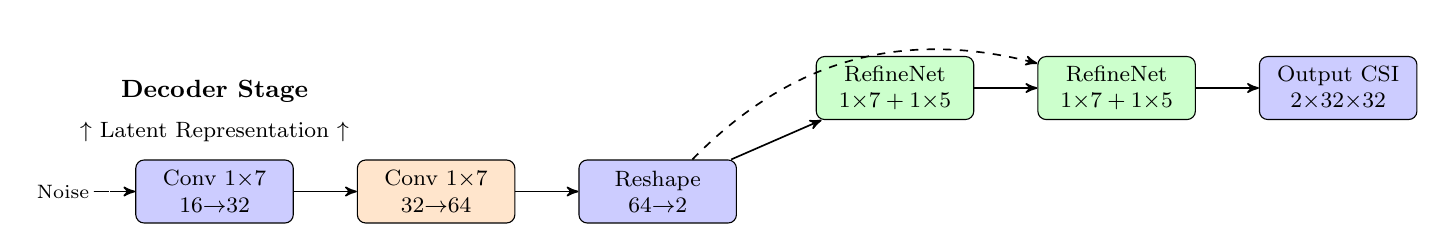
\begin{tikzpicture}[
    node distance=0.5cm and 0.8cm,
    block/.style={draw, fill=white, rectangle, minimum width=2cm, minimum height=0.8cm, font=\footnotesize, align=center, rounded corners=3pt},
    conv/.style={block, fill=orange!20},
    residual/.style={block, fill=green!20},
    compress/.style={block, fill=blue!20},
    arrow/.style={->, >=stealth', semithick}
]

% Latent Space Exit
\node[compress] (decoder1) {Conv $1{\times}7$ \\ $16{\rightarrow}32$};
\node[conv, right=of decoder1] (decoder2) {Conv $1{\times}7$ \\ $32{\rightarrow}64$};
\node[compress, right=of decoder2] (reshape2) {Reshape \\ $64{\rightarrow}2$};

% RefineNet
\node[residual, above right=0.5cm and 1cm of reshape2] (refine1) {RefineNet \\ $1{\times}7+1{\times}5$};
\node[residual, right=of refine1] (refine2) {RefineNet \\ $1{\times}7+1{\times}5$};

% Output
\node[compress, right=of refine2] (output) {Output CSI \\ $2{\times}32{\times}32$};

% Continuation Marker
\node[above=0.1cm of decoder1, font=\footnotesize] {$\uparrow$ Latent Representation $\uparrow$};

% Arrows
\draw[arrow] (decoder1) -- (decoder2);
\draw[arrow] (decoder2) -- (reshape2);
\draw[arrow] (reshape2) -- (refine1);
\draw[arrow] (refine1) -- (refine2);
\draw[arrow] (refine2) -- (output);

% Skip connections
\draw[arrow, dashed] (decoder1.west) to[out=180,in=180] node[pos=0.6, left] {\scriptsize Noise} (-1.5,0) to (decoder1.west);
\draw[arrow, dashed] (reshape2) to[bend left] (refine2);

% Part label
\node[above=0.6cm of decoder1, font=\small\bfseries] {Decoder Stage};
\end{tikzpicture}

\caption{Complete CLLWCsiNet architecture: (Upper) Encoder stage with multi-scale feature extraction and latent space compression. (Lower) Decoder stage with reconstruction and denoising refinement. The $\gamma$ denotes compression ratio options.}
\label{fig:complete_arch}
\end{figure*}

\end{document}